In this section, we first formulate the multivariate time series anomaly detection problem. We then present the architecture of CATS and provide a detailed description of each of its components. In particular, we explain the data augmentation techniques employed in our work, introduce and describe the temporal contrastive loss, and the global contrastive loss. Finally, we define the computation of the anomaly score, which is utilized for the detection of time series anomalies.

\subsection{Problem Formulation}

Given a multivariate time series dataset $X = \{x_1,x_2, ..., x_T\}$, where $T$ is the length of $X$ and $x_t \in \mathbb{R}^m$ denotes a $m$-dimensional vector corresponding to the values of our $m$ features at time $t$. The dataset is sliced into sequences of time series windows $W = \{w_1, w_2, ..., w_{T-p+1}\}$ with stride 1 where $w_t = \{x_t, x_{t+1}, ..., x_{t+p-1}\} \in \mathbb{R}^{p \times m}$, $p$ being the window size.

Time series anomaly detection aims at training an unsupervised anomaly detection model $\mathcal{M}$ that given an unknown window time series $\tilde{w_t}$ at inference time will output an anomaly score $s(\tilde{w_t})$. By using this anomaly score and a threshold $\eta$,  a binary label $\tilde{y_t} \in \{0,1\}$ is computed which indicates whether a window is anomalous ($\tilde{y_t} = 1$) or not ($\tilde{y_t} = 0$).


\begin{figure*}[!t]
  \centering
  \begin{tabular}{@{}c@{}}
  %\label{fig:chap_5:training}
    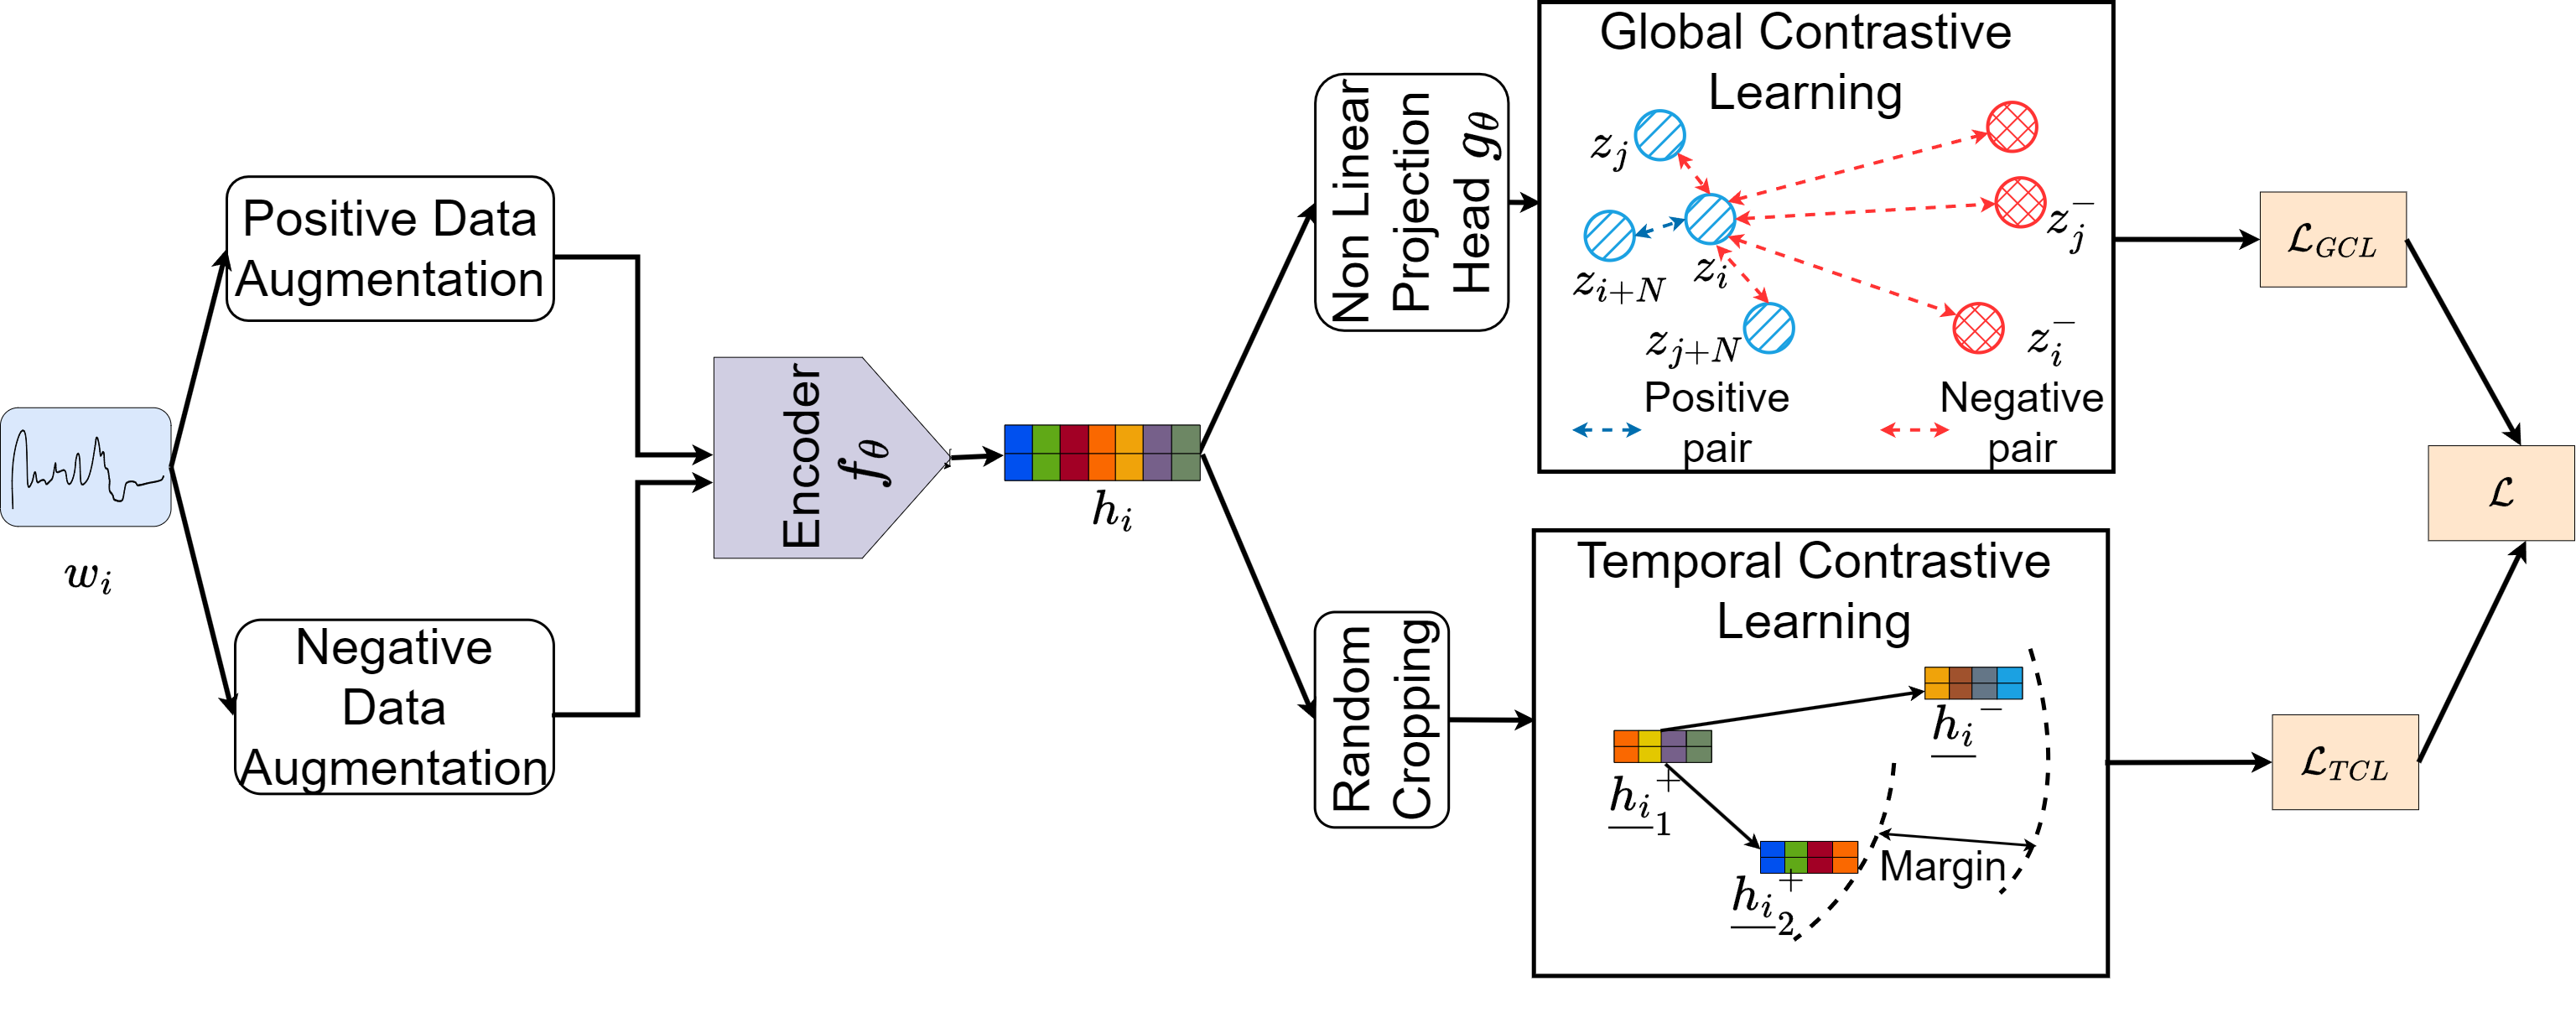
\includegraphics[width=.8\linewidth]{imgs/chapter_5/train.png} \\[\abovecaptionskip]
    \small (a) Training
  \end{tabular}

  \vspace{\floatsep}

  \begin{tabular}{@{}c@{}}
  %\label{fig:chap_5:inference}
    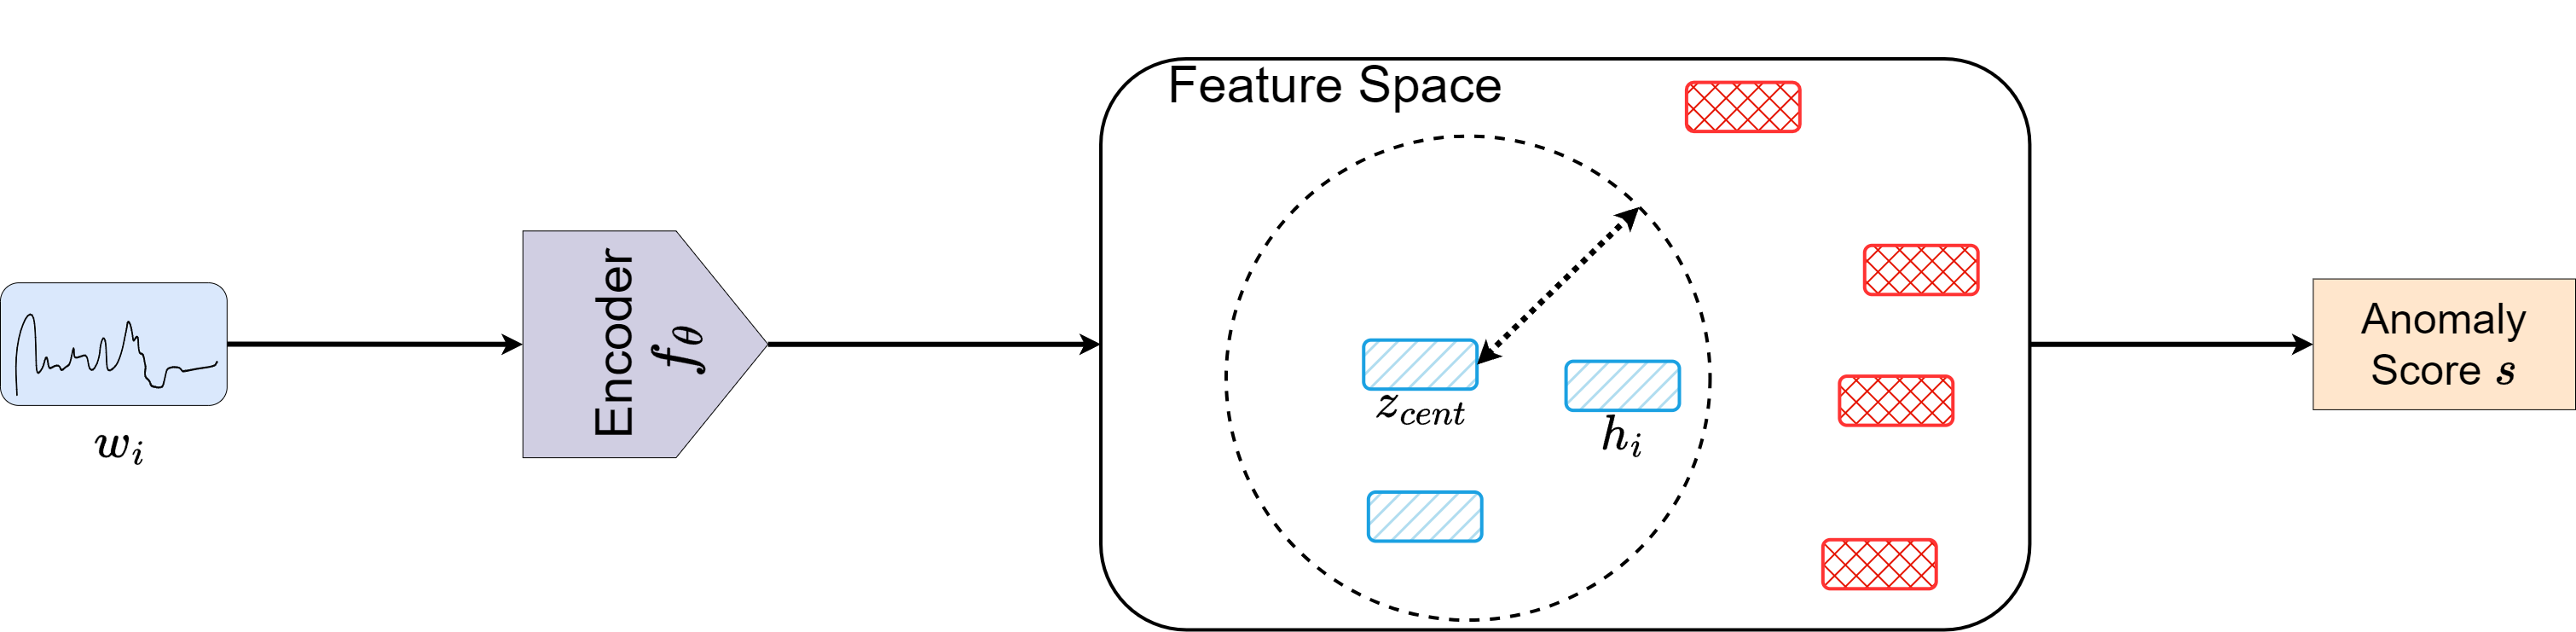
\includegraphics[width=.8\linewidth]{imgs/chapter_5/inference.png} \\[\abovecaptionskip]
    \small (b) Inference
  \end{tabular}
  \caption{The proposed architecture of CATS. (a) is the training phase which consists in time series representation learning with temporal contrastive learning (TCL) and global contrastive learning (GCL). (b) is the inference phase where given an unknown window time series $\tilde{w_i}$ its anomaly score is computed as the distance between its latent representation $\tilde{h_i}$ and the centroid of training samples $z_{cent}$.}
  \label{fig:chap_5:architecture}
\end{figure*}



\subsection{Model Architecture}
The overall architecture of CATS is shown in Fig. \ref{fig:chap_5:architecture}. Our architecture comprises the following components:
\begin{itemize}
    \item A stochastic data augmentation module that transforms each input window time series $w_i$ to three views: two positive views $\{w_i^{+}; w_{i+N}^{+}\}$ and a negative view $w_i^{-}$.
    \item A siamese network encoder $f_{\theta}$ that learn representations from augmented views of the input window time series $h_i = f_{\theta}(w_i) \in \mathbb{R}^{p \times d}$ with $d$ the feature size.
    \item A projection head $g_{\theta}$ that projects the latent representations $h_i$ to a projection space $z_i = g_{\theta}(h_i)$ due to its importance for contrastive learning \cite{chen2020simple}.
    \item A global contrastive loss (GCL) that performs contrastive learning on projection space giving the set of $(z_i)$ from the batch using an improvement of NT-Xent loss \cite{Sohn2016ImprovedDM}.
    \item Random cropping is applied on feature space representations $h_i$ to built temporal pairs for the temporal contrastive learning.
    \item A temporal contrastive loss (TCL) to enforce temporal similarity between cropped versions $(\underline{h_i} \in \mathbb{R}^{k \times d})$ ($k$ the crop size) of latent vectors and a triplet loss.

\end{itemize}

The model is trained using a contrastive loss model combining the temporal and the global contrastive losses defined as follows:

\begin{equation}\label{loss_total}
    \mathcal{L} = \alpha . \mathcal{L}_{TCL} + \beta . \mathcal{L}_{GCL}
\end{equation}
where $\alpha$ and $\beta$ are two hyper-parameters representing the relative weight of each loss. %\abdelkader{Pourquoi ces valeurs de 0.5, ce serait bien d'expliquer!}

At inference time, the projector $g_{\theta}$ is discarded and a anomaly score is obtained by computing the distance between an unseen window and the center of latent representations.

\subsection{Data augmentation}
Data augmentation plays a crucial role in contrastive learning, facilitating the learning process. While diverse data augmentation techniques are available in the computer vision domains, selecting appropriate data augmentation methods for time series remains challenging. Building upon previous works that have utilized or evaluated data augmentation for time series \cite{chen2020simple, Iwana2020AnES}, we define a set of positive data augmentations $\mathcal{D}_{aug}^{+} = \{d_1^+, \ldots, d_{n_{aug}^+}\}$ which are as follows, given a window time series $w = (x_1, \ldots, x_p)$:
\begin{itemize}
    \item Jitter transformation adds a i.i.d Gaussian noise with zero mean and variance $\sigma^2$ to the time series.
        \begin{equation}
            d_{jitter}(w) = w + \mathcal{N}(0, \sigma^2)
        \end{equation}
    \item Scaling transformation changes the global magnitude of a portion $P$ of the time series by multiplying all the values by a scaling factor $\alpha$.
        \begin{equation}
            d_{scaling}(w) = \alpha_{scaling} * w_P
        \end{equation}
\end{itemize}


In the context of unsupervised learning for anomaly detection, the focus is typically on modeling normality using only normal instances during training, and anomalous instances are only encountered during inference. We use negative data augmentations to incorporate weak supervision during the representation learning stage, thus providing prior information about what does not constitute normal data \cite{DARBAN2025110874, kim2023contrastive, li2023contrastive, sinha2021negative}. This approach enhances the learning process by incorporating knowledge of abnormal patterns during training. We thus define a a set of negative data augmentations $\mathcal{D}_{aug}^{-} = \{d_1^-, \ldots, d_{n_{aug}^-}\}$ which are as follows:

\begin{itemize}
    % \item Spike transformation simulates point anomalies by applying extreme values spikes to randomly selected points of the time series.
    %     \begin{equation}
    %         d_{spike}(w) = (\widehat{x_1}, ..., \widehat{x_p}) \\
    %         \text{ with } \widehat{x_i} = x_i . a
    %     \end{equation}
    \item Mask transformation consists in randomly masking some points of the time series.
        \begin{equation}
            d_{mask}(w) = (\widehat{x_1}, \ldots, \widehat{x_p}) \\
            \text{ with } \widehat{x_i} = 0
        \end{equation}
    % \item Shuffle transformation divides the time series window into $k$ sub-sequences and permute them.
    %     \begin{equation}
    %         d_{shuffle}(w) = \pi(w_{1: \lfloor \frac{p}{2} \rfloor}, ..., w_{ (k-1)\lfloor \frac{p}{k} \rfloor: p} )
    %     \end{equation}
    \item Trend transformation applies a linear drift $w_{drift}$ to the time series to simulate a shift in the trend of the time series.
        \begin{equation}
            d_{trend}(w) = w + w_{drift}
        \end{equation}
\end{itemize}

Thus, given a time series window $w_i$ from a batch $\mathcal{B}$ of size $N$, we generate two positive views $w_i^{+}$ and $w_{i+N}^{+}$ and one negative view $w_i^{-}$ resulting in a batch of positive samples $\mathcal{B}^{+} = (w_i^{+})_{i=1}^{2N}$ and a batch of negative samples $\mathcal{B}^{-} = (w_i^{-})_{i=1}^{N}$.

However, the range of anomalies present in time series data is usually large, and it is not feasible to expect negative data augmentations to generate all possible anomalies. Therefore, similar to previous studies \cite{DARBAN2025110874, kim2023contrastive, li2023contrastive}, random data augmentation is employed. Specifically for each window $w_t$, and a selected data augmentation $d_i^- \in \mathcal{D}_{aug}^{-}$, diversity is enforced through the hyperparameters of $d_i$ that control the augmentation process. These hyperparameters include the ratio of features $n_{feat}$ that will be augmented and the ratio of time points $n_{t}$ that will be augmented per features. Given $n_{feat}$ (resp. $n_{t}$), and a given time series window $w_t$, a random subset of features (resp. time steps) will be chosen for augmentation. This approach allows for increased variability and diversity in the generated augmented samples, enhancing the learning process for anomaly detection in multivariate time series data.

\subsection{Temporal Contrastive Learning}
One shortcoming of previous anomaly detection approaches using contrastive learning is that they do not exploit temporal dependencies for contrasting. We address this limitation by proposing a novel Temporal Contrastive Loss (TCL). TCL aims at learning temporal properties, and clusters time series window that are temporally similar while pushing away windows that are dissimilar. To achieve that representation in the feature space, we use DTW (Dynamic Time Warping) \cite{sakoe1971dynamic} as a time series similarity measure that is more suited for time series forecasting or clustering than classical Euclidean distance.

DTW similarity measure aims at minimizing the Euclidean distance between aligned time series under all possible temporal alignments. However, DTW measure is not differentiable and is not suitable for gradient-based algorithms. To overcome this limitation, Soft-DTW \cite{Cuturi2017SoftDTWAD} was proposed to smooth DTW and make it differentiable everywhere and then can be used as a loss function or similarity measure. In this work, we choose a Soft-DTW variant called Soft-DTW divergence \cite{blondel2021differentiable}  that unlike the former is positive and minimized when the time series are equal. Specifically given two time series $x_i$ and $x_j$, Soft-DTW divergence is defined as follows:

\begin{equation}\label{soft_dtw_div}
\begin{split}
    D^{\gamma}(x_i, x_j) &= DTW_{Soft}^{\gamma}(x_i, x_j)  \\ 
    &- \frac{1}{2} (DTW_{Soft}^{\gamma}(x_i, x_i) + DTW_{Soft}^{\gamma}(x_j, x_j))
\end{split}
\end{equation}
with $DTW_{Soft}^{\gamma}(.)$ being the Soft-DTW measure and $\gamma$ a smoothing parameter.

To enhance the temporal contrastive learning, we build triplets using cropped versions (subsets of time series windows as defined in \cite{Yue2021TS2VecTU}) of the two positive views and a crop version of the negative view. Specifically, we apply random cropping on a positive view $h_i^+ \in \mathbb{R}^{p \times d}$ to generate two positive subseries $\underline{h_i}_1^+$ and $\underline{h_i}_2^+ \in \mathbb{R}^{k \times m}$ where $k < p$. We do the same process on a negative view $h_i^-$ to obtain a negative subseries $\underline{h_i}^-$.  The rationale behind building triplets in this way, instead of using the views resulting from positive and negative data augmentations to build them, is to ensure that the two positive subseries will be \textit{temporally} similar and \textit{temporally} distant from the negative subseries. Since we consider only normal time series windows to build positive pairs, we avoid the limitation of the cropping strategy raised by \cite{Yue2021TS2VecTU}.

%This cropping strategy may be inefficient if there exists level shifts in the same time series window, as raised by \cite{Yue2021TS2VecTU}. However, in our anomaly detection task this is not the case since the training set contains only normal windows.

Given this similarity measure, and a triplet of latent representations $\{\underline{h_i}_1^+; \underline{h_i}_2^+; \underline{h_i}^-\}$ TCL is defined as follows:

\begin{equation}\label{temp_loss}
    \mathcal{L}_{TCL} = \frac{1}{N} \sum_{i=1}^{N} max(D^{\gamma}(\underline{h_i}_1^+ - \underline{h_i}_2^+) - D^{\gamma}(\underline{h_i}_1^+ - \underline{h_i}^-) + m; 0)
\end{equation}
where $D^{\gamma}(.)$ is the Soft-DTW divergence measure, $m$ the margin (minimum distance that must be kept between positive samples and negative samples). One advantage of Soft-DTW divergence measure is that it can be applied to time series of different sizes and then our TCL can be computed using the cropped versions of the latent vectors. However, the computation of Soft-DTW has a quadratic time complexity which can increase the training time.


\subsection{Global Contrastive Learning}
We define a Global Contrastive Loss to learn representations at the instance level. This loss improves the NT-Xent loss by considering more negative pairs for contrastive learning. Traditionally, given an instance $z_i$ in a batch of size $N$, CL models using this loss contrast one positive pair $(z_i, z_i^+)$ i.e., two views from the same instance to $N-1$ negative pairs $(z_i, z_j^{+})$ $\forall j \neq i$ i.e., pairs with views of different instances. 

However, in anomaly detection tasks that are performed on normality assumptions, the training data mostly belong to the same class, i.e., normal data. To enhance, the representation learning, we include views coming from negative data augmentation. Specifically, we form a negative pairs by computing the similarity between an instance and all negative views of all the instances in the batch $(z_i, z_j^{-})$ $\forall j \in [|1;N|]$. Consequently, we get one positive pair and $2N-1$ negative pairs for each $z_i$ in the batch. Then, the GCL is expressed as follows:


\begin{equation}\label{gcl_loss}
    \mathcal{L}_{GCL} = \frac{1}{2N} \sum_{i \in \mathcal{B}^{+}} log \frac{exp(sim(z_i, z_{i+N})/\tau)}{\sum_{j \in \mathcal{B} \text{ and } j \neq i} exp(sim(z_i, z_j)/\tau)}
\end{equation}
with $\mathcal{B} = \mathcal{B}^{+} \cup \mathcal{B}^{-}$, $N$ the batch size, $\tau$ the temperature hyperparameter and $sim(.)$ the cosine similarity.

\begin{equation}\label{sim}
    sim(z_i, z_j) = \frac{z_i . z_j^{T}}{\|z_i\|\|z_j\|}
\end{equation}

\subsection{Anomaly score}\label{sec:anomaly}
After model training, we discard the projection head $g_{\theta}$ and we only use the encoder $f_{\theta}$ for our downstream task since $h_i$ feature have more information for contrastive learning than $z_i$ \cite{chen2020simple}. To identify anomalies, we follow the same assumptions as one-class classifiers and we expect the normal data to be clustered and anomalies to lies away from that cluster. Hence, given a window from the test set $\tilde{w_t}$, we define the anomaly score $s(.)$ as follows:

\begin{equation}\label{score}
\begin{split}
    s(\tilde{w_t}) &= \mathcal{D}(f_{\theta}(\tilde{w_t}), z_{cent}) =  \mathcal{D}(\tilde{z_t}, z_{cent})
\end{split}
\end{equation}

\begin{equation}
    z_{cent} = \frac{1}{N_{train}} \sum_{i=1}^{N_{train}} w_i
\end{equation}
where $\mathcal{D}(.)$ is the L2-distance measure function, $z_{cent}$ is the centroid of latent features of the training set and $N_{train}$ is the size of the training set. 

One advantage of using Eq. \ref{score} as anomaly score is that $z_{cent}$ can be computed offline and stored allowing lower inference time.

